\documentclass{article}
\usepackage{graphicx}
\usepackage[utf8]{inputenc}
\usepackage[T1]{fontenc}
\usepackage{fouriernc}
\usepackage[margin=1in]{geometry}
\usepackage{amsmath}
\begin{document}

\begin{titlepage}
	\centering 
	\scshape
	\vspace*{\baselineskip}
	\rule{\textwidth}{1.6pt}\vspace*{-\baselineskip}\vspace*{2pt}
	\rule{\textwidth}{0.4pt} 
	\vspace{0.75\baselineskip}
	
	{\Large CS 374 : Computational and Numerical Methods \\\vspace{0.75\baselineskip} Set 16}
	\vspace{0.75\baselineskip}
	
	\rule{\textwidth}{0.4pt}\vspace*{-\baselineskip}\vspace{3.2pt} 
	\rule{\textwidth}{1.6pt}
	
	\vspace{2\baselineskip}  
	Runge-Kutta Method
	
	\vspace*{3\baselineskip}
	
	\vspace{0.5\baselineskip} %originally 0.5
	
	{\scshape\large Purvil Mehta (201701073) \\ Bhargey Mehta (201701074) \\} 
	
	\vspace{1\baselineskip} 
	
	\textit{Dhirubhai Ambani Institute of Information and Communication Technology \\ Gandhinagar\\} 
	\vspace*{2\baselineskip}
	\today


\end{titlepage}

\newpage

\section{$Y'(X) = -Y(X) + 2\cos{X}$ with $Y(0) = 1$}
\begin{figure}[!h]
    \centering
    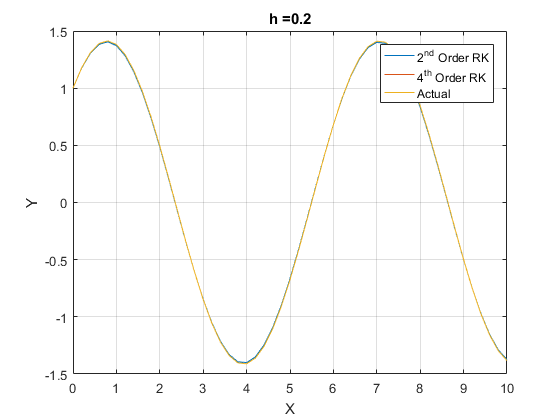
\includegraphics[scale = 0.55]{16_1.png}
    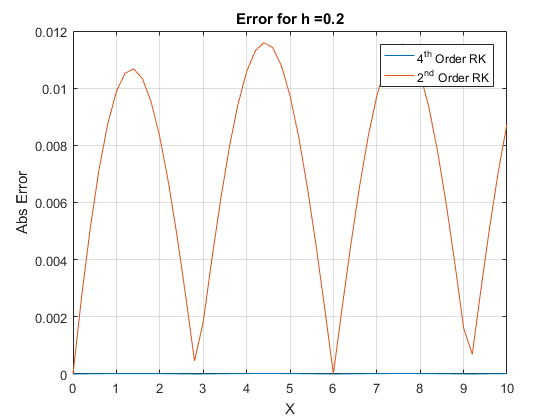
\includegraphics[scale = 0.55]{16_2.png}
    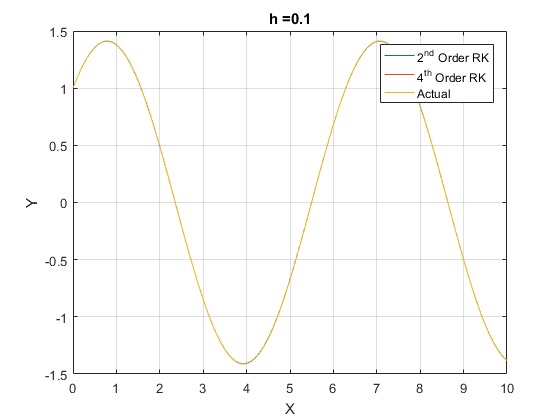
\includegraphics[scale = 0.55]{16_3.png}
    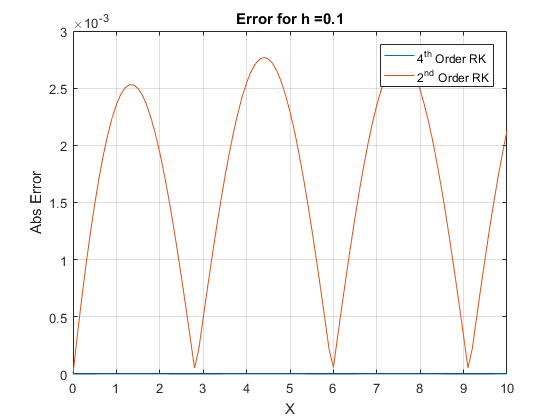
\includegraphics[scale = 0.55]{16_4.png}
    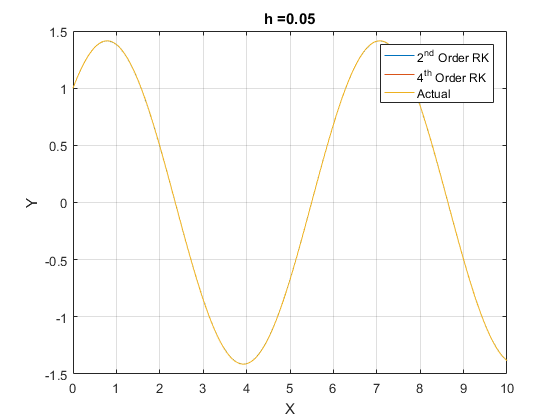
\includegraphics[scale = 0.55]{16_5.png}
    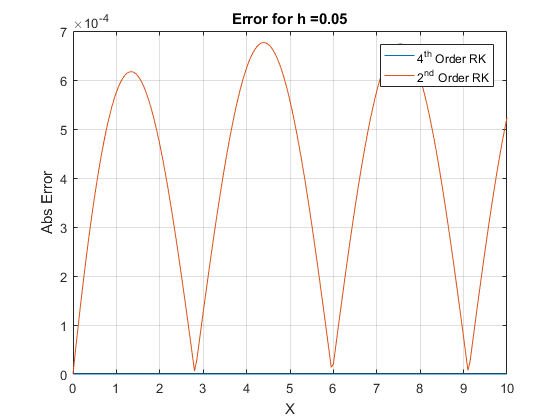
\includegraphics[scale = 0.55]{16_6.png}
    \caption{Comparison of the First Order and the Second Order Runge Kutta Method Method}
\end{figure}

\newpage
\section{$Y'(X) = -Y(X) + X^{0.1}(1.1+X)$ with $Y(0) = 0$}
\begin{figure}[!h]
    \centering
    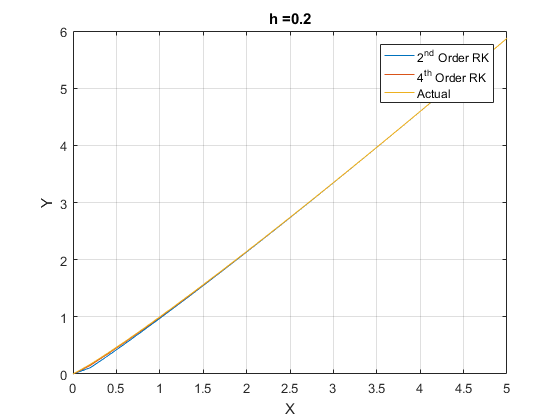
\includegraphics[scale = 0.55]{16_1_2.png}
    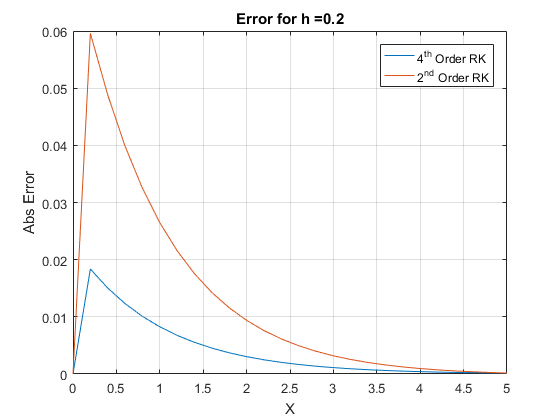
\includegraphics[scale = 0.55]{16_2_2.png}
    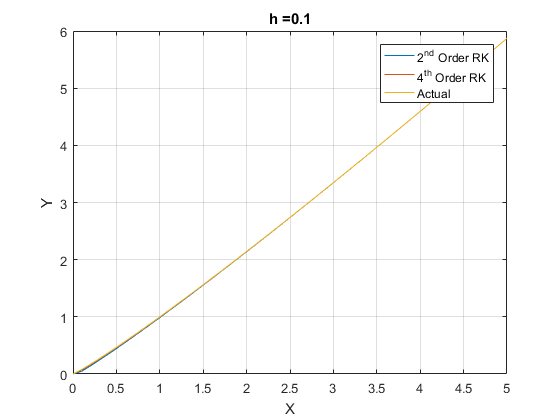
\includegraphics[scale = 0.55]{16_3_2.png}
    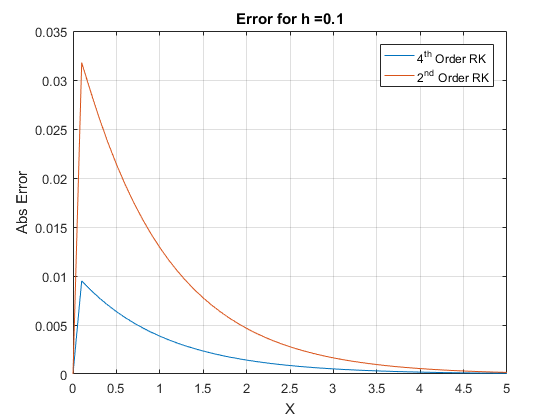
\includegraphics[scale = 0.55]{16_4_2.png}
    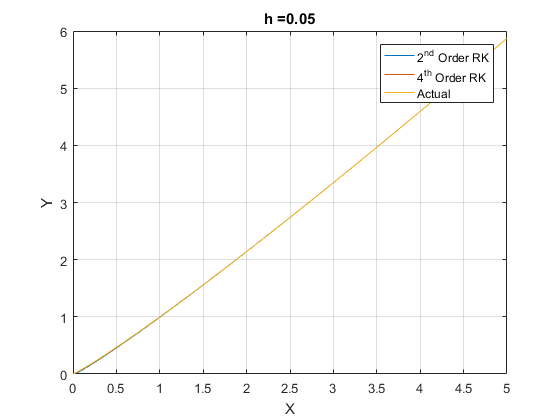
\includegraphics[scale = 0.55]{16_5_2.png}
    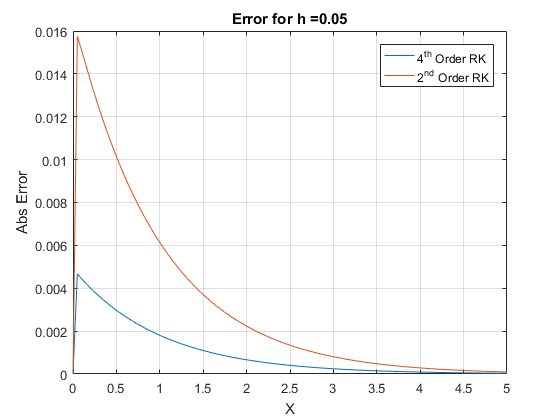
\includegraphics[scale = 0.55]{16_6_2.png}
    \caption{Comparison of the First Order and the Second Order Runge Kutta Method Method}
\end{figure}

\newpage
\section{$Y'(X) = -Y(X) + X^{0.1}(1.1+X)$ with $Y(0) = 0$}
\begin{figure}[!h]
    \centering
    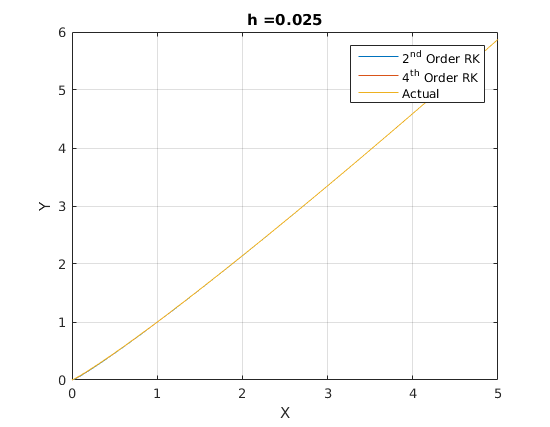
\includegraphics[scale = 0.5]{x_1.png}
    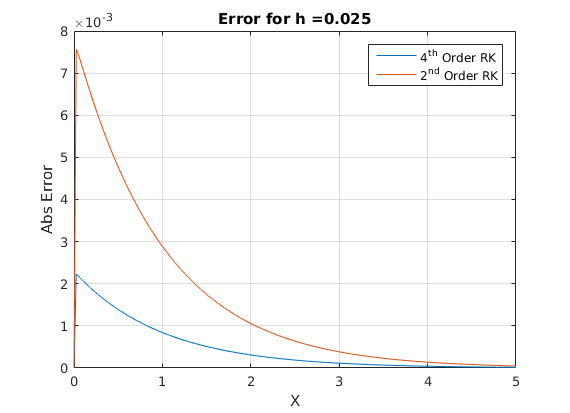
\includegraphics[scale = 0.5]{x_1_e.png}
    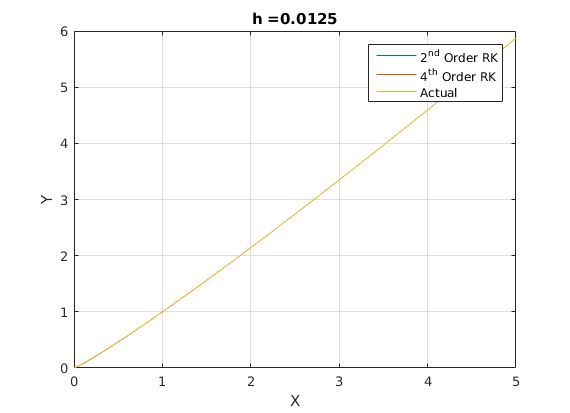
\includegraphics[scale = 0.5]{x_2.png}
    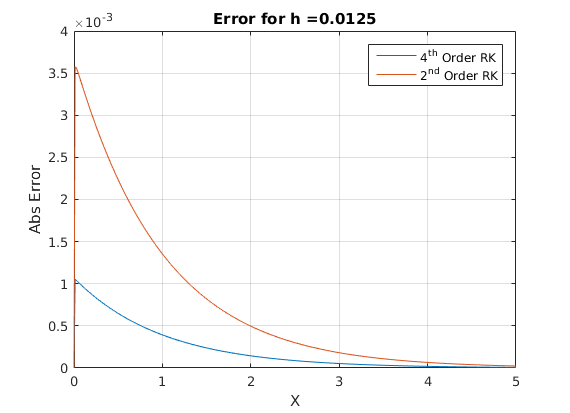
\includegraphics[scale = 0.5]{x_2_e.png}
    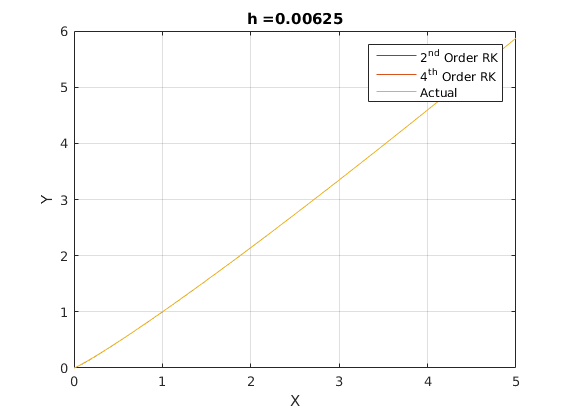
\includegraphics[scale = 0.5]{x_3.png}
    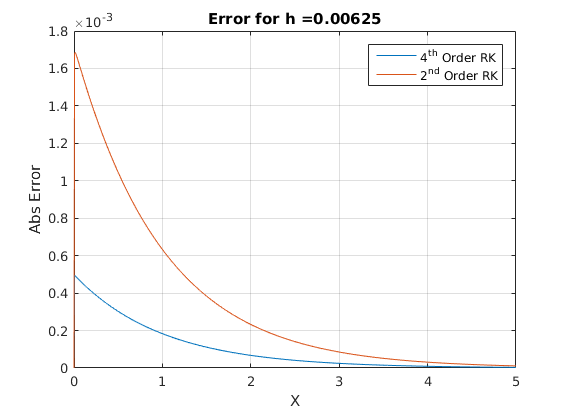
\includegraphics[scale = 0.5]{x_3_e.png}
    \caption{Comparison of the First Order and the Second Order Runge Kutta Method Method}
\end{figure}
\end{document}